\documentclass[tikz, border = 5pt]{standalone}
\usetikzlibrary{quotes,angles}
\usepackage{tkz-euclide}
\usetkzobj{all}
\begin{document}
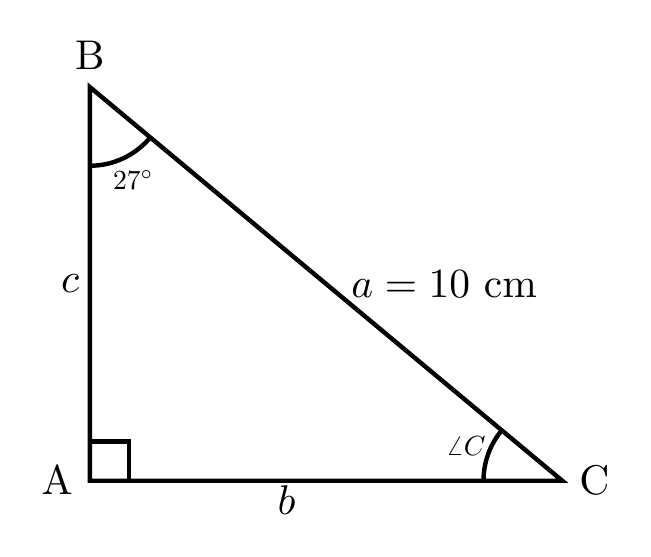
\begin{tikzpicture}
  \draw[ultra thick]
    (6,0) coordinate (a) node[right, scale=1.5] {C}
    -- (0,0) coordinate (b) node[left, scale=1.5] {A}
    -- (0,5) coordinate (c) node[above, scale=1.5] {B}
   -- cycle
    pic["$\angle C$", draw=black, angle eccentricity=1.3, angle radius=1cm]
    {angle=c--a--b}
    pic["$27^\circ$", draw=black, angle eccentricity=1.3, angle radius=1cm]
    {angle=b--c--a};
   \tkzMarkRightAngle[ultra thick, draw=black, size=.5](c,b,a);

  \node[scale=1.5] at (2.5,-.25) {$b$};
  \node[scale=1.5] at (-.25,2.5) {$c$};
  \node[scale=1.5] at (4.5,2.5) {$a = 10 \mbox{ cm}$};

\end{tikzpicture}
\end{document}
